\section{Budget}\label{appendix_budget}

In order to keep track of the used money in the project, a budget was created for the project. The budget is sepperated in testing phase and final product cost, in order to track the budget against the goals set in the project. In cases there was ordered spares or replacements hence the quantity difference in the final product cost and testing phase. 

\begin{figure}[H]
    \begin{center}
    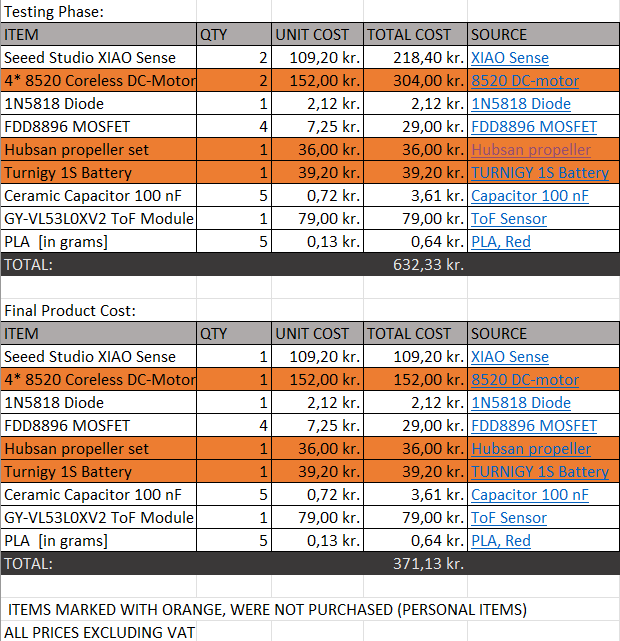
\includegraphics[scale=0.7]{pictures/Budget.png}
    \end{center}
    \caption{Budget for the semester project}
    \label{fig:Surge_Current}
\end{figure}

